\subsubsection{Light-quark contributions}

\label{EW:light-quark}

%\paragraph{Authors:}
%\begin{itemize}
%    \item Marco Bonetti, Philipp Rendler, William J. Torres Bobadilla~\cite{Bonetti:2025vfd,BoHeReToBa_TBA};
%    \item Arunima Bhattacharya, Francisco Campanario, Sauro Carlotti, Jamie Chang, Javier Mazzitelli, Margarete Mühlleitner, Jonathan Ronca, Michael Spira ~\cite{Bhattacharya_TBA}.
%\end{itemize}


\begin{figure}
\centering
    \subfloat[$VVh$]{{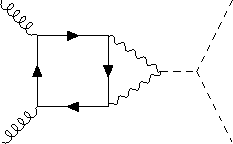
\includegraphics[height=0.10\textheight]{NLO_EW_SM/EW_light_quarks/Images/gg-HHH}}\label{fig:VVHV}}
	\qquad\qquad
    \subfloat[$VVhh$]{{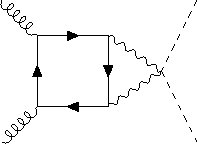
\includegraphics[height=0.10\textheight]{NLO_EW_SM/EW_light_quarks/Images/gg-HHVV}}\label{fig:HHVV}}
	\qquad\qquad
    \subfloat[$VVV$]{{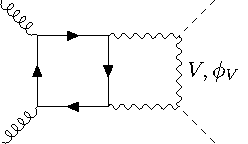
\includegraphics[height=0.10\textheight]{NLO_EW_SM/EW_light_quarks/Images/gg-VVV}}\label{fig:VVV}}
	\caption{Representative diagrams for the light-quark contributions from Ref.~\cite{Bonetti:2025vfd}.}
    \label{fig:amplgg}
\end{figure}


Double Higgs boson production in gluon fusion mediated by light quarks appears for the first time at two loops: the gluons couple to a light-quark box, to which either two $W$ or two $Z$ bosons are attached, subsequently generating the Higgs boson(s). Three blocks of contributions can be identified: one-particle reducible diagrams containing one vector-vector-Higgs vertex and one trilinear Higgs boson self-coupling vertex (dubbed $VVH$, see Fig.~\ref{fig:VVHV}); diagrams containing a vector-vector-Higgs-Higgs vertex ($VVHH$, Fig.~\ref{fig:HHVV}); and diagrams containing two vector-vector-Higgs vertices ($VVV$, Fig.~\ref{fig:VVV}).\footnote{The $VVV$ type of diagrams may also contain a Goldstone boson connecting the two Higgs bosons.} Each one of these blocks is further divided into diagrams containing either $W$ or $Z$ bosons only. Each one of the aforementioned terms is explicitly gauge-invariant and UV- and IR-finite. Four light flavours are considered in diagrams containing $W$ bosons, while five light flavours have been taken into account in diagrams containing $Z$ bosons.

~

\noindent \textbf{Marco Bonetti, Philipp Rendler, William Torres Bobadilla~\cite{Bonetti:2025vfd}.}

\noindent In Ref.~\cite{Bonetti:2025vfd} fully symbolic expressions for each of the blocks described above have been calculated. The amplitude has been decomposed as a linear combination of the standard tensors $T_1^{\mu\nu}$ and $T_2^{\mu\nu}$ of Section~\ref{intro_ampli}.\footnote{No axial terms are generated by the fermion loop thanks to charge-parity conservation.}

The two form factors are extracted, and the set of scalar two-loop Feynman integrals appearing there is reduced to master integrals. Differential equations are derived for specific linear combinations of the master integrals with respect to the Mandelstam variables and the masses, such that their solution can be written in terms of iterated integrals over logarithmic kernels. This choice of basis is further improved by applying a series of rotations to eliminate redundant integration kernels. Integration constants are fixed by matching the expressions of the master integrals to their large-$m_{W,Z}$ expansion.

The results are employed to obtain analytic expressions for the form factors, further identifying independent functions therein for which dedicated differential equations are built for optimized numerical evaluation in terms of generalized series expansions evolved from the large-mass limit to arbitrary points in the physical region of the phase space. A code implementation for the numerical evaluation of the functions is provided, based on the \texttt{Mathematica} package \texttt{DiffExp}~\cite{Hidding:2020ytt}. Grids for the light-quark amplitude, as well as for its interference with the LO amplitude, have been implemented in the POWHEG-BOX framework or are available upon request. The interference between the LO amplitude and the first form factor of the light-quark amplitude represents the main source of contributions except for the high-energy tail, where the second form factor becomes relevant, although very small overall. Large cancellations occur when considering the interference between LO triangle and box diagrams with each of the $VVh$, $VVhh$, and $VVV$ blocks, suggesting that the light-quark terms are highly sensitive to variations of the trilinear Higgs boson self-coupling.


\begin{figure}
\centering
    \subfloat[]{{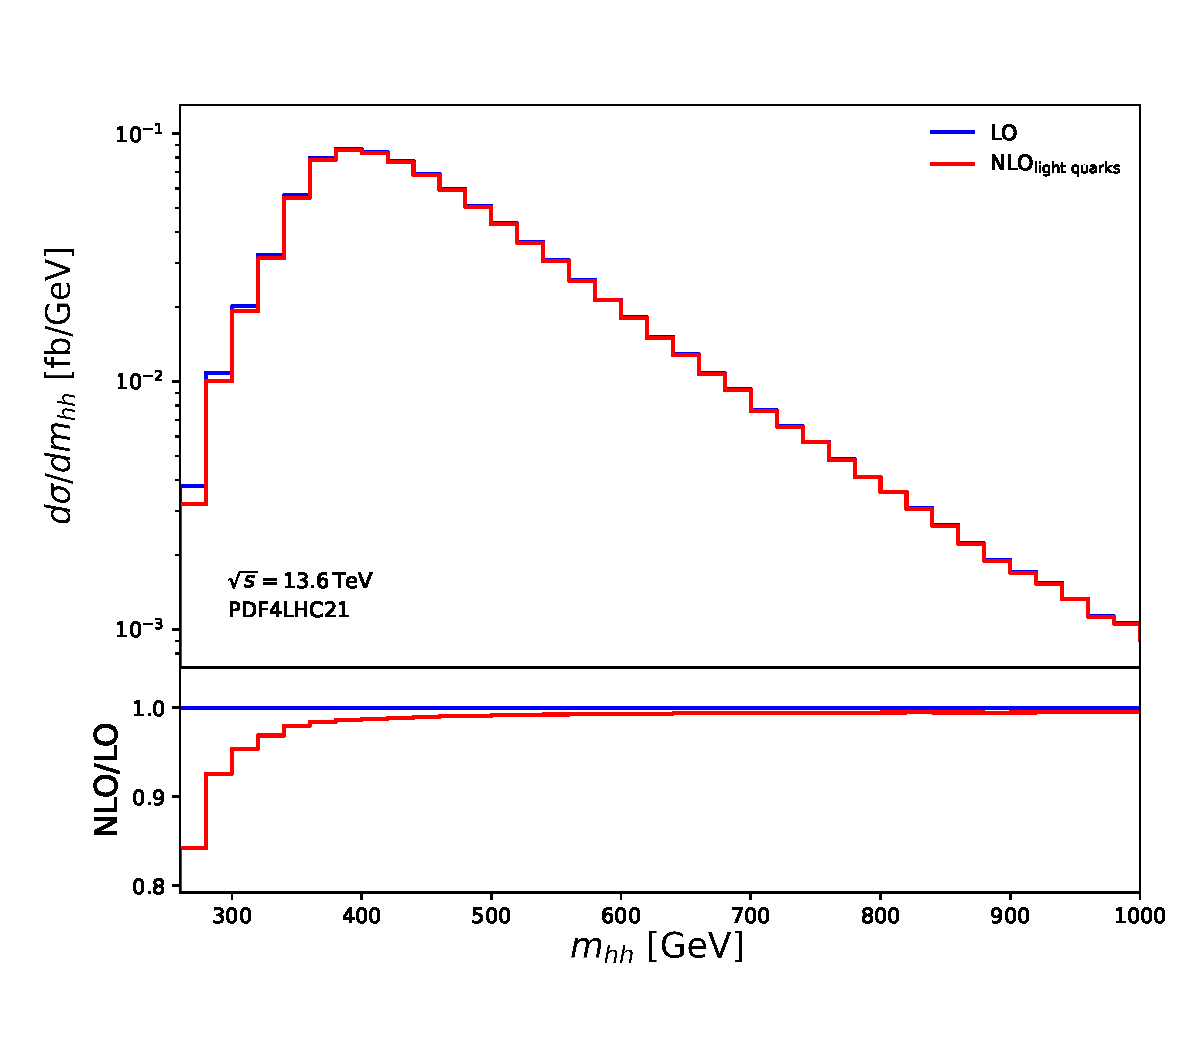
\includegraphics[width=0.48\textwidth]{NLO_EW_SM/EW_light_quarks/Images/mhh2_hfix.pdf}}\label{fig:lq_mHH}}
	\quad
    \subfloat[]{{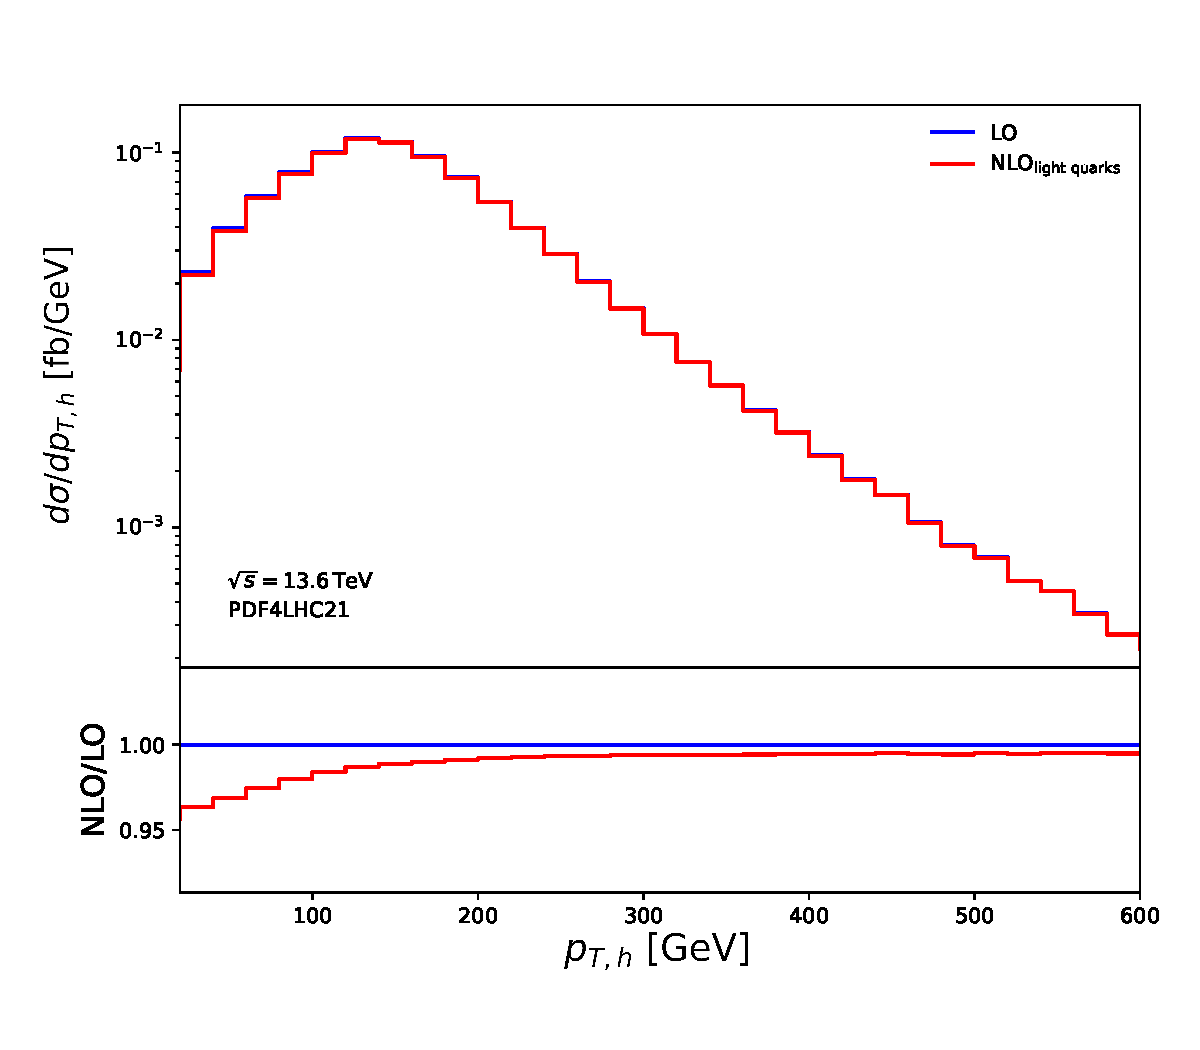
\includegraphics[width=0.48\textwidth]{NLO_EW_SM/EW_light_quarks/Images/pt_hfix.pdf}}\label{fig:lq_pTH}}
	\caption{Light-quark and Yukawa contributions to the Higgs boson pair invariant mass (a) and Higgs transverse momentum distributions (b).}
    \label{fig:lq_obs}
\end{figure}


The impact of the light-quark corrections to the Higgs boson pair invariant mass distribution and the transverse momentum distribution is depicted in Figs.~\ref{fig:lq_mHH} and~\ref{fig:lq_pTH}, respectively. The light-quark corrections suppress both the invariant mass and the transverse momentum distribution at all centre-of-mass energies, with particular relevance for the region of the phase space close to the production threshold, where they have a negative effect of more than $-15\%$ on the $m_{hh}$ distribution and around $-4\%$ on the $p_{T,h}$ distribution. In both cases, the corrections quickly approach zero as the centre-of-mass energy grows.

~

\noindent \textbf{Arunima Bhattacharya, Francisco Campanario, Sauro Carlotti, Jamie Chang, Javier Mazzitelli, Milada Margarete Mühlleitner, Jonathan Ronca, Michael Spira ~\cite{Bhattacharya_TBA}.}

\noindent Ref.~\cite{Bhattacharya_TBA} provides an independent evaluation of the light-quark contributions to $gg \to hh$. The bottleneck of this calculation is the evaluation of the genuine two-loop box diagrams $VVV$ (see Fig.~\ref{fig:VVV}). The numerical stability of these diagrams is quite demanding, since strong cancellations emerge between all diagrams, which require the form factors of the individual diagrams to be numerically determined with very significant precision. The numerical method applied to these diagrams is the same as in Section~\ref{EW:Top-Higgs_sector}, i.e.\ projection on the two form factors of Eq.~\eqref{eq:FFdeco} in $D=4-2\epsilon$ dimensions, no tensor reduction, Feynman parametrization and analytical continuation of all propagator masses including the $W$ and $Z$ boson masses, $M_{W/Z}^2 \to M_{W/Z}^2 (1-i\bar\epsilon)$. To isolate the singularities, multiple end-point subtractions need to be performed. In order to reach the narrow-width limit $\bar\epsilon\to 0$, a Richardson extrapolation was performed with a minimal regulator down to $\bar\epsilon = 0.025$ depending on $m_{hh}$.

The two-loop triangle diagrams $VVh$ (see Fig.~\ref{fig:VVHV}) can be adopted from the single-Higgs calculation \cite{Aglietti:2004nj,Aglietti:2006yd} and translated to the two-loop box diagrams with a 4-point vertex $VVhh$ (see Fig.~\ref{fig:HHVV}).


\begin{figure}[!hbtp]
    \centering
   % \vspace*{-3.2cm}
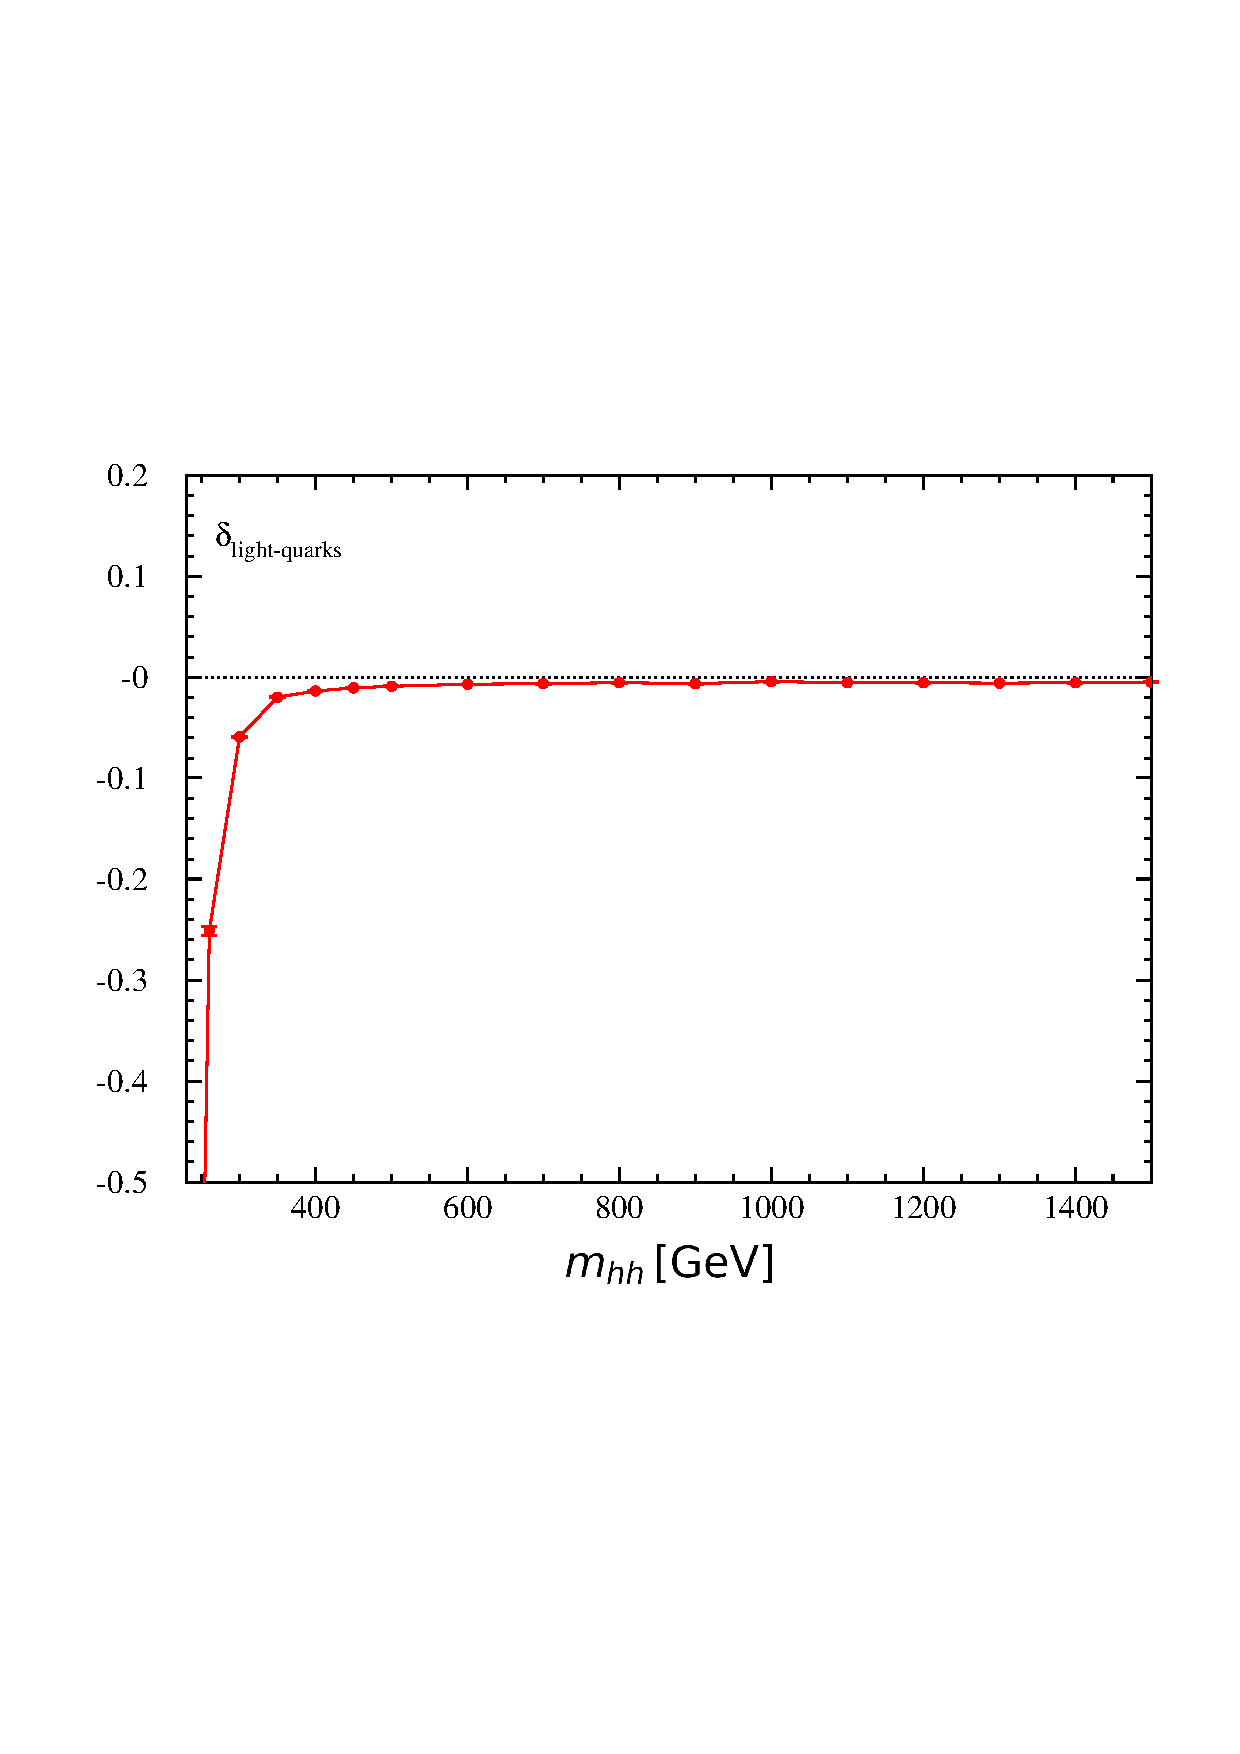
\includegraphics[width=0.48\textwidth]{NLO_EW_SM/EW_light_quarks/Images/delta_lq_hfix.pdf}
 %   \vspace*{-3.2cm}
\caption{\label{fg:delta_lq}The full relative light-quark loop-induced electroweak corrections to the $gg \to hh$ process. The points on the curve together with their numerical error bars indicate the $m_{hh}$ values for which the corrections have been computed. Results shown are from Ref.~\cite{Bhattacharya_TBA}.}
\end{figure}


The total sum of all light-quark loop diagrams is finite, and no renormalization is required. The result is a small correction at the sub-percent level for large values of $m_{hh}$, see Fig.~\ref{fg:delta_lq}, while the corrections are larger close to the production threshold due to the cancellation of the leading top quark mass terms of the LO matrix element, to which the results are normalized. In total, the light-quark loops do not play a dominant role in Higgs boson pair production via gluon fusion in contrast to single-Higgs production \cite{Actis:2008ts,Actis:2008ug}.

~

\paragraph{Comparison.}

The two independent evaluations of the light-quark contributions mentioned above have been found to agree within the numerical uncertainties.
